\documentclass{beamer}
\mode<presentation>{
  \usetheme{Warsaw}
}

\usepackage[makeroom]{cancel}
\usepackage{mathtools}
\newcommand{\defeq}{\vcentcolon=}
\newcommand{\eqdef}{=\vcentcolon}

\usepackage{graphicx}

\usepackage{tikz-qtree}
\usepackage{gb4e}

\title[ Parsing MGAs ]{ Adjunction in Minimalist Grammars }
\subtitle{ Parsing with Fowlie's MGA Formalism }
\author[ \texttt{pmn25} ]{ Patrick Niedzielski \texttt{pmn25} }

\begin{document}

\begin{frame}
  \titlepage
\end{frame}

\AtBeginSection[]
{
\begin{frame}{}
\tableofcontents[currentsection]
\end{frame}
}

\section{Background}
\subsection{Minimalist Grammars}

\begin{frame}{The Minimalist Program}
  Chomsky (1995). \textit{The Minimalist Program}.
  
  \begin{center}
    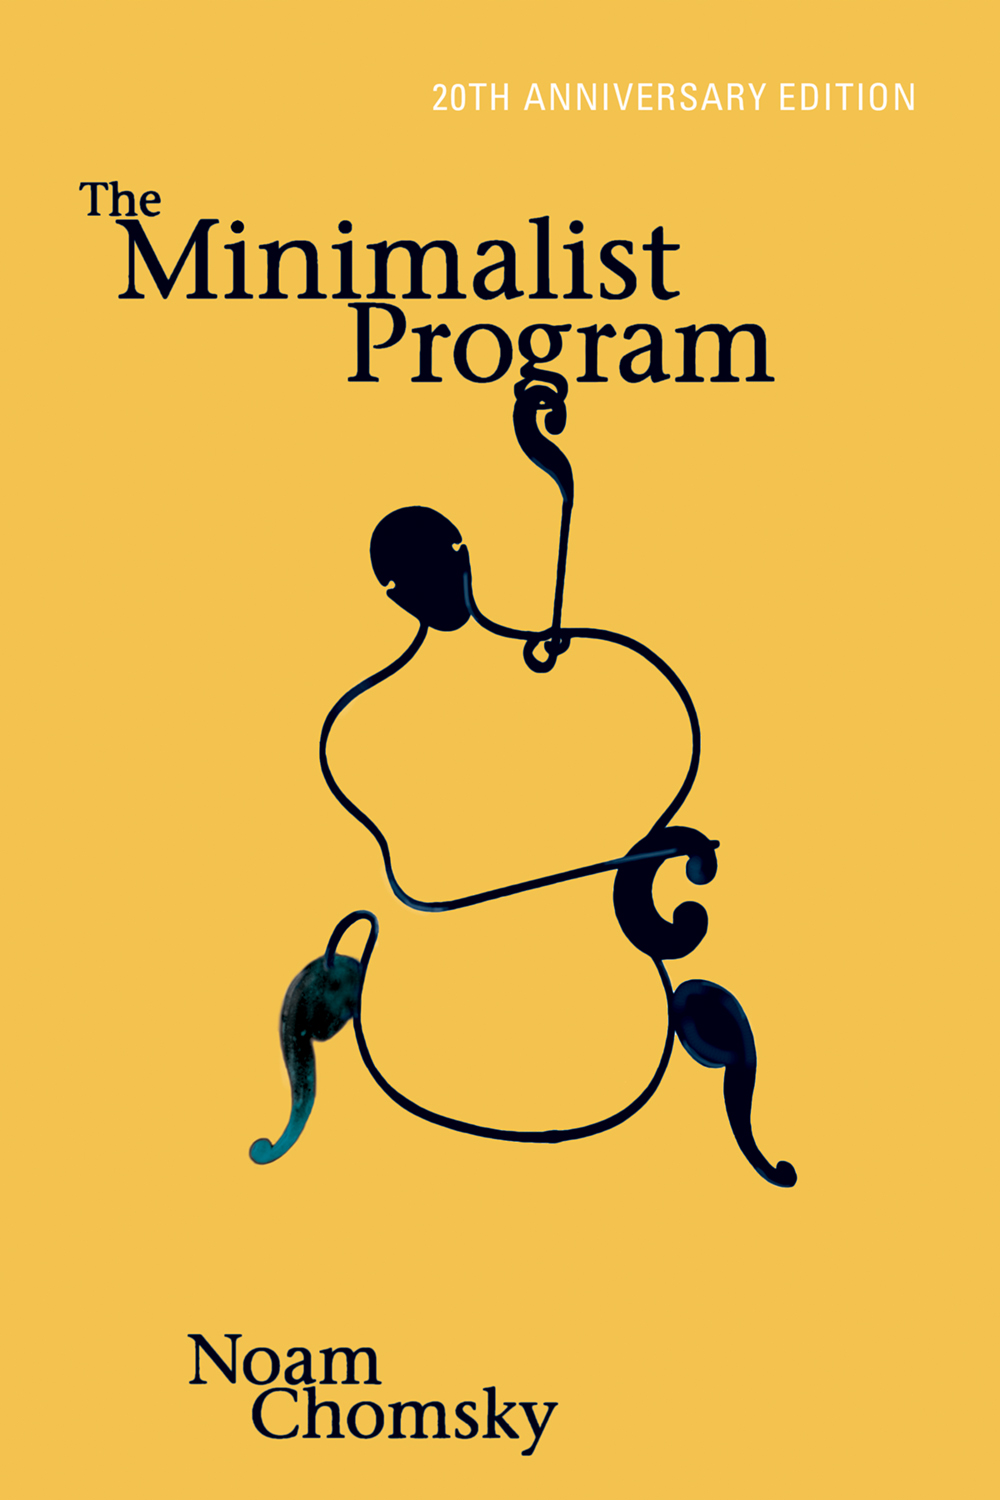
\includegraphics[width=0.3\textwidth]{minimalist-program}
  \end{center}
\end{frame}

\begin{frame}{Minimalist Program}
  Two fundamental operations:

  \begin{columns}
    \column{0.5\textwidth}
    \begin{block}{Merge}
      (Or External Merge)

      \[
        Merge( \alpha, \beta ) \defeq \{ \alpha \{ \alpha, \beta \} \}
      \]

      \begin{center}
        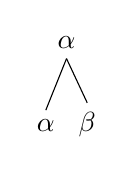
\begin{tikzpicture}
          \Tree[.$\alpha$ $\alpha$ $\beta$ ]
        \end{tikzpicture}
      \end{center}
    \end{block}

    \column{0.5\textwidth}
    \begin{block}{Move}
      (Or ReMerge, Internal Merge)

      \begin{center}
        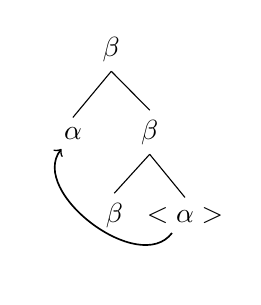
\begin{tikzpicture}
          \Tree[.$\beta$ \node(y){$\alpha$}; [.$\beta$ $\beta$ \node(x){$<\alpha>$}; ] ]
          \draw[semithick, ->] (x) to [bend left=90] (y);
        \end{tikzpicture}
      \end{center}
    \end{block}
  \end{columns}
\end{frame}

\begin{frame}{Minimalist Grammars}
  \begin{itemize}
  \item Minimalism is motivated by a computational perspective, but it
    is not computationally rigorous.
  \item Ed Stabler built a formalization of the Minimalist Program,
    called \textbf{Minimalist Grammars}, where all derivation is the
    result of checking features on atoms.
    \pause
  \item Merge checks \textbf{selectional features}, allowing atoms
    with features \texttt{F} and \texttt{=F} to merge, with the latter
    as the head.
  \item Move checks \textbf{licensing features}, discontiguous
    allowing atoms with features \texttt{-F} and \texttt{+F} to merge,
    with the latter as the head.
  \end{itemize}
\end{frame}

\begin{frame}{Minimalist Grammars}
  Two operations:

  \begin{columns}
    \column{0.5\textwidth}
    \begin{block}{Merge}
      \begin{center}
        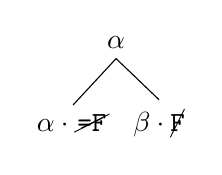
\begin{tikzpicture}
          \Tree[.$\alpha$ $\alpha \cdot \cancel{\texttt{=F}}$ $\beta \cdot \cancel{\texttt{F}}$ ]
        \end{tikzpicture}
      \end{center}
    \end{block}

    \column{0.5\textwidth}
    \begin{block}{Move}
      \begin{center}
        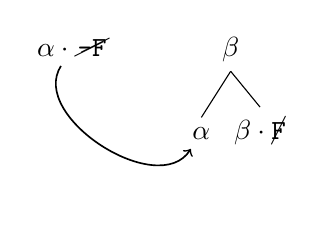
\begin{tikzpicture}
          \Tree[.\node(x){$\alpha \cdot \cancel{\texttt{-F}}$}; ]
          \begin{scope}[xshift=2cm]
            \Tree[.$\beta$ \node(y){$\alpha$}; $\beta \cdot \cancel{\texttt{F}}$ ] ]
          \end{scope}
          \draw[semithick, ->] (x) to [bend right=90] (y);
        \end{tikzpicture}
      \end{center}
    \end{block}
  \end{columns}
\end{frame}

\begin{frame}{Minimalist Grammars}
  \begin{center}
    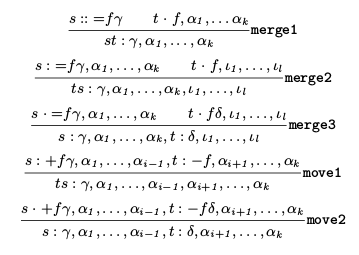
\includegraphics[width=0.5\textwidth]{mg-inference-rules}
  \end{center}
\end{frame}

\subsection{Chart Parsing}

\begin{frame}{CKY Recognition}
  \begin{itemize}
  \item A recognition algorithm for context free grammars in Chomsky
    Normal Form.
  \item There are two parts to the CKY recognition algorithm:
    \begin{enumerate}
    \item the \textbf{chart}, which contains all derivations we know
      to be valid at a given point during the algorithm, and
    \item the \textbf{agenda}, which contains all derivations we will
      try to use to form new derivations.
    \end{enumerate}
  \item The recognition algorithm initializes the agenda and chart
    with lexical items in the input string, and then searches for new
    derivations by looping through the agenda.
  \item Recognition succeeds if we find one of the goal items in the
    chart.
  \end{itemize}
\end{frame}

\begin{frame}{Chart Parsing through Inference Rules}
  This can also be thought of as application of inference rules, which
  allows us to generalize from CFGs to arbitrary consistent logics!
\end{frame}

\section{Motivation}

\subsection{Adjunction}
\begin{frame}{Adjunction}
  \pause
  \begin{center}
    \Huge Adjunction is hard.
  \end{center}
\end{frame}

\begin{frame}{Adjunction}
  \begin{exe}
    \ex[]{The (bad) wolf.}
    \ex[]{The bad, bad, bad wolf.}
    \ex[]{\atcenter{
      \arrowalign{The&\ bad&\ wolf.\cr
        \fillright\vrule&\lf&\fillleft\pu\cr}
    }}
    \ex[]{The big, bad wolf.}
    \ex[*]{The bad, big wolf.}
    \ex[]{I saw the man in the street with the gun.}
    \ex[]{I saw the man with the gun in the street.}
    \ex[]{\atcenter{
        \arrowalign{Bright&\ blue&\ balloon.\cr
          \fillright\vrule&\centr{\pu\spacer\vrule}&\fillleft\pu\cr}
      }}
    \ex[]{He is clever.}
  \end{exe}
\end{frame}

\begin{frame}{Hornstein}
  \begin{center}
    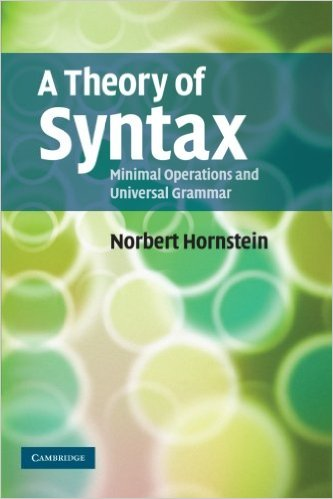
\includegraphics[width=0.4\textwidth]{theory-of-syntax}
  \end{center}
\end{frame}

\begin{frame}{Adjunction in Minimalist Grammars?}
  \begin{itemize}
  \item Is it possible with Minimalist Grammars, though? \pause
  \item To get recursion, optionality, and transparency to selection,
    we could stipulate that adjuncts have features \texttt{=FF}---that
    is, they select for an \texttt{F} and yield an \texttt{F}.
  \item But now the adjunct is the new head of the phrase.
  \item We also can't get adjunction with strict ordering.
  \item It seems the best we can do is massive homophony in the
    lexicon to get all the features.
  \end{itemize}
\end{frame}

\begin{frame}{Adjunction in Minimalist Grammars?}
  \begin{itemize}
  \item \textbf{Can we do better?}
  \item Idea: Implement a parser for Minimalist Grammars (or slightly
    modified MGs) that can handle adjunction correctly.
  \end{itemize}
\end{frame}

\section{Minimalist Grammars with Adjunction}

\begin{frame}{Fowlie's MGAs}
  Meaghan Fowlie, in her dissertation, creates a new formalism called
  \textbf{Minimalist Grammars with Adjunction} that is weakly
  equivalent to Stabler's Minimalist Grammar formalism (derives the
  same set of languages).
\end{frame}

\begin{frame}{Adjoin}
  Let's keep Merge and Move as they are, but introduce a new
  operation, Adjoin:

  \begin{block}{Adjoin}
    \begin{center}
        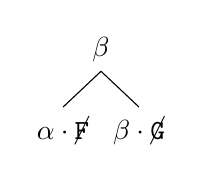
\begin{tikzpicture}
          \Tree[.$\beta$ $\alpha \cdot \cancel{\texttt{F}}$ $\beta \cdot \cancel{\texttt{G}}$ ]
        \end{tikzpicture}
      \end{center}
  \end{block}

  Very similar to Merge, so we can use very similar inference rules!
\end{frame}

\begin{frame}{Adjoin}
  \begin{itemize}
  \item To prevent anything from adjoining to anything, we add to the
    grammar a mapping from a category to the categories that are
    allowed to adjoin with it.  For instance,

    \[
      Ad(\mathtt{N}) = \{ \mathtt{A} \}
    \]
  \item To allow ordering of adjuncts, we instrument our category and
    selection features with the maximum level an adjunct can adjoin
    to, and and the level of the entire phrase.
    \begin{itemize}
    \item Thus, if \textit{big} has category \texttt{[A, 3, 0]} and
      \textit{bad} has category \texttt{[A, 5, 0]}, we rule out
      *\textit{bad big wolf}, because we'd be merging something of
      category \texttt{[A, 3, 0]} with something of category
      \texttt{[N, 0, 5]}, and $5 > 3$.
    \end{itemize}
  \end{itemize}
\end{frame}


\section{Progress}

\begin{frame}{Implementation Strategy}
  \begin{enumerate}
  \item Implement chart parser for Minimalist Grammars using the
    inference rules shown before.
  \item Create inference rules for Minimalist Grammars with Adjunction
    based on Fowlie's dissertation.
  \item Extend parser with the new inference rules.
  \end{enumerate}
\end{frame}

\begin{frame}{Progress}
  \begin{itemize}
  \item Only a recognizer right now.
  \item Several false starts with recognizing MGs.
  \item Once MG parser was finished, though, MGAs have been relatively
    easy to implement.
  \item Inference rules for adjunction are very similar to those for
    merging.
  \item Currently recursive adjuncts are rejected---not good!
  \end{itemize}
\end{frame}


\end{document}

%%% Local Variables:
%%% mode: latex
%%% TeX-master: t
%%% End:
